% STATUS: ACTIVE -- 2026-11-03 (user): new document of the local estimator, layout of 1029 (loose). Section 1 = angle update, result
%   relations only (derivation in 1029). No Q, R, gate, no curvature (user 11-03). Notation as 1026 / 1029: delta-theta-hat_u, _v, _w =
%   small angles about the local axes of V-hat[k]; left superscript V[k] = local coordinate of V-hat[k]; a-hat_22 = a-hat_11 for now, written as a-hat_11 (user 11-03: separate a_22 only after the simulation checks); Sections 2, 3 copied from 1026 Sections 2, 4 without the grey notes (user 11-03); macros from 1026. Section 4 = 1026 Section 4 (dynamics of estimation errors) without the grey notes; Section 5 Regulation (user 11-03): PI, tau_P (P part, = tau_a of 1021 and the code) and tau_I (I part, code tau_i), tau_I = 4 tau_P; slope floor and integration-start condition of the code not written. Section 6 control force variance (user 11-04): one axis, gain known, fixed point, delay 2, measured position fed back (upper bound for the KF); figure from test_script/scratch/run_1104_force_var.m.
%   Code: test_script/scratch/run_t3_xyz_fixed.m, local arm: dth (angle step, ~line 789), V-hat rebuilt from the angles (~801),
%   positions rotated with C = V-hat'[k+1] V-hat[k] (~809), a_11, a_33 kept and a_13, a_23 from the rotated matrix (~805, 11-01 fix).
% Compile: xelatex 1103_angle_update.tex (from reference/eq17_analysis/derivation/).
\documentclass[11pt,a4paper]{ctexart}
\usepackage[fleqn]{amsmath}
\usepackage{amssymb,bm,upgreek,graphicx}
\setlength{\mathindent}{0pt}
\usepackage{geometry}
\geometry{margin=1.8cm}
\setlength{\parindent}{0pt}
\setlength{\parskip}{0.2em}
\AtBeginDocument{\setlength{\abovedisplayskip}{10pt}\setlength{\belowdisplayskip}{10pt}}
\setlength{\jot}{8pt}
\renewcommand{\arraystretch}{1.35}
\usepackage{xcolor}
\graphicspath{{figures/}}
\newcommand{\setline}[1]{\par\medskip\noindent{\small\textcolor[gray]{0.35}{#1}}}
\newcommand{\hd}[1]{\par\bigskip\noindent\underline{\textbf{#1}}}
% fonts: upright Greek scalars, bold upright vectors / matrices
\newcommand{\lc}{\lambda_c}
\newcommand{\dl}{\delta}
\newcommand{\bth}{\bm{\uptheta}}
\newcommand{\bep}{\bm{\upvarepsilon}_p}
\newcommand{\Lb}{\bar{\bm{\Lambda}}}
\newcommand{\Sn}{\bm{\Sigma}_n}
\newcommand{\Ab}{\bar{\mathbf A}}
\newcommand{\Ah}{\hat{\mathbf A}}
\newcommand{\Am}{\bar{\mathbf A}_m}
\newcommand{\av}{\bar{\mathbf a}}
\newcommand{\ah}{\hat{\mathbf a}}
\newcommand{\am}{\bar{\mathbf a}_m}
\newcommand{\dpb}{\dl\bar{\mathbf p}}
\newcommand{\dph}{\dl\hat{\mathbf p}}
\newcommand{\Fd}{\bar{\mathbf F}_{dp}}
\newcommand{\Mb}{\mathbf M}
\newcommand{\Mh}{\hat{\mathbf M}}
\newcommand{\I}{\mathbf I}
\newcommand{\V}{\mathbf V}
\newcommand{\Vh}{\hat{\mathbf V}}
\newcommand{\uu}{\mathbf u}
\newcommand{\vv}{\mathbf v}
\newcommand{\ww}{\mathbf w}
\newcommand{\wh}{\hat{\mathbf w}}
\newcommand{\apar}{\bar a_{11}}
\newcommand{\aper}{\bar a_{33}}
\newcommand{\CK}{C_T\,\kappa_T}
\newcommand{\E}{\mathrm{E}}
\newcommand{\T}{T}
\newcommand{\GA}{\begin{bmatrix} F_x & 0 & 0 & F_y & F_z & 0 \\ 0 & F_y & 0 & F_x & 0 & F_z \\ 0 & 0 & F_z & 0 & F_x & F_y \end{bmatrix}}
\newcommand{\Jt}{\dfrac{\partial\bth}{\partial\av}\bigg|_{\Ah}}
\newcommand{\eyl}[1]{\big[\,\mathbf e_p^{\T}[k]\ \ \mathbf e_a^{\T}[k]#1\,\big]^{\T}}
\newcommand{\nv}{\big[\,\mathbf 0\ \ \mathbf 0\ \ -\bep^{\T}[k]\ \ \big(\hat{\mathbf a}'[k]\,\wh^{\T}[k]\,\bep[k]\big)^{\T}\ \ \mathbf 0\ \ \mathbf 0\,\big]^{\T}}
\newcommand{\Jw}{\dfrac{\partial\ww}{\partial\bth}\bigg|_{\hat\bth}}
\newcommand{\vA}{{}^{v}\bar{\mathbf A}}
\newcommand{\vAh}{{}^{v}\hat{\mathbf A}}
\newcommand{\vAm}{{}^{v}\bar{\mathbf A}_m}
\newcommand{\vdp}{{}^{v}\dl\bar{\mathbf p}}
\newcommand{\vdph}{{}^{v}\dl\hat{\mathbf p}}
\newcommand{\vF}{{}^{v}\bar{\mathbf F}_{dp}}
\newcommand{\vM}{{}^{v}\mathbf M}
\newcommand{\vMh}{{}^{v}\hat{\mathbf M}}
\newcommand{\vep}{{}^{v}\bm{\upvarepsilon}_p}
\newcommand{\dd}{\big(\apar - \aper\big)}
\newcommand{\ddh}{\big(\hat a_{11} - \hat a_{33}\big)}
\newcommand{\dth}{\delta\hat\theta}
\newcommand{\ef}{\big[\,\mathbf e_p^{\T}[k]\ \ \mathbf e_a^{\T}[k]\,\big]^{\T}}
\pagestyle{plain}

\begin{document}

\section{Angle update}

\vspace{1.2em}
\begin{align*}
{}^{V[k]}\Ab[k+1] &\approx \begin{bmatrix} \hat a_{11}[k+1] & 0 & \hat a_{13}[k+1] \\ 0 & \hat a_{11}[k+1] & \hat a_{23}[k+1] \\ \hat a_{13}[k+1] & \hat a_{23}[k+1] & \hat a_{33}[k+1] \end{bmatrix}
\end{align*}

\vspace{2.2em}
\begin{align*}
\dth_u[k] &= \frac{\hat a_{23}[k+1]}{\hat a_{11}[k] - \hat a_{33}[k]} \\[4pt]
\dth_v[k] &= -\frac{\hat a_{13}[k+1]}{\hat a_{11}[k] - \hat a_{33}[k]} \\[4pt]
\dth_w[k] &= -\tan\hat\theta_x[k]\,\dth_v[k]
\end{align*}

\vspace{2.2em}
\begin{align*}
\hat\theta_x[k+1] &= \hat\theta_x[k] + \dth_u[k] \\[4pt]
\hat\theta_y[k+1] &= \hat\theta_y[k] + \frac{\dth_v[k]}{\cos\hat\theta_x[k]}
\end{align*}

%======================================================================
\clearpage
\section{Process in the local coordinate}
\vspace{1.2em}
\begin{align*}
\vA &= \Vh^{\T}\,\Ab\,\Vh = \begin{bmatrix} \apar & 0 & \bar a_{13} \\ 0 & \apar & \bar a_{23} \\ \bar a_{13} & \bar a_{23} & \aper \end{bmatrix} \\
\bar a_{23} &= \dd\big(\theta_x - \hat\theta_x\big) \\
\bar a_{13} &= -\dd\cos\hat\theta_x\,\big(\theta_y - \hat\theta_y\big)
\end{align*}
\vspace{1.2em}
\begin{align*}
{}^{v}\bar{\mathbf f}_d[k] &= \vAh^{-1}[k]\,\Big\{{}^{v}\bar{\mathbf p}_d[k+1] - {}^{v}\hat{\mathbf p}[k] - \lc\,\big({}^{v}\bar{\mathbf p}_d[k] - {}^{v}\hat{\mathbf p}[k]\big)\Big\}
\end{align*}
\vspace{1.2em}
\begin{align*}
\vdp[k+1] &= \lc\,\vdp[k] - \big(\vA - \vAh[k]\big)\,\vF[k] - \vep[k] \\
\big(\vA - \vAh\big)\,\vF &= \mathbf G_a[k]\,\big[\,\apar - \hat a_{11}\ \ \aper - \hat a_{33}\ \ \bar a_{13} - \hat a_{13}\ \ \bar a_{23} - \hat a_{23}\,\big]^{\T} \\
\mathbf G_a[k] &= \begin{bmatrix} F_u & 0 & F_w & 0 \\ F_v & 0 & 0 & F_w \\ 0 & F_w & F_u & F_v \end{bmatrix}
\end{align*}
\vspace{1.2em}
\begin{align*}
\vM[k] &= {}^{v}\Delta\bar{\mathbf p}_d[k] + (1-\lc)\,\vdp_3[k] \\
{}^{v}\ww &= \big[\,\cos\hat\theta_x\,(\theta_y - \hat\theta_y)\ \ \ -(\theta_x - \hat\theta_x)\ \ \ 1\,\big]^{\T}
\end{align*}
\vspace{1.2em}
\begin{align*}
\vdp_1[k+1] &= \vdp_2[k] \\
\vdp_2[k+1] &= \vdp_3[k] \\
\vdp_3[k+1] &= \lc\,\vdp_3[k] - \big(\vA - \vAh[k]\big)\,\vF[k] - \vep[k] \\
\apar[k+1] &= \apar[k] + \apar'[k]\;{}^{v}\ww^{\T}\Big(\vM[k] + \big(\vA - \vAh[k]\big)\,\vF[k] + \vep[k]\Big) \\
\aper[k+1] &= \aper[k] + \aper'[k]\;{}^{v}\ww^{\T}\Big(\vM[k] + \big(\vA - \vAh[k]\big)\,\vF[k] + \vep[k]\Big) \\
\apar'[k+1] &= \apar'[k] \\
\aper'[k+1] &= \aper'[k] \\
\bar a_{13}[k+1] &= \bar a_{13}[k] \\
\bar a_{23}[k+1] &= \bar a_{23}[k] \\
\bth[k+1] &= \bth[k]
\end{align*}

%======================================================================
\clearpage
\section{Estimator}
\vspace{1.2em}
\begin{align*}
&\big[\,\vdp_1^{\T}\ \ \vdp_2^{\T}\ \ \vdp_3^{\T}\ \ \apar\ \ \aper\ \ \apar'\ \ \aper'\ \ \bar a_{13}\ \ \bar a_{23}\ \ \theta_x\ \ \theta_y\,\big]^{\T} \qquad (17 \times 1,\ d = 2)
\end{align*}
\vspace{1.2em}
\begin{align*}
{}^{v}\dpb_m[k] &= \Vh^{\T}[k]\,\dpb_m[k], \qquad \vAm[k] = \Vh^{\T}[k]\,\Am[k]\,\Vh[k] \\
\bar a_{m,11} &= \tfrac{1}{2}\Big(\big[\vAm\big]_{11} + \big[\vAm\big]_{22}\Big), \qquad \bar a_{m,33} = \big[\vAm\big]_{33}, \qquad
\bar a_{m,13} = \big[\vAm\big]_{13}, \qquad \bar a_{m,23} = \big[\vAm\big]_{23}
\end{align*}
\vspace{1.2em}
\begin{align*}
\mathbf y_m[k] &= \begin{bmatrix} {}^{v}\dpb_m[k] \\ \bar a_{m,11}[k] \\ \bar a_{m,33}[k] \\ \bar a_{m,13}[k] \\ \bar a_{m,23}[k] \end{bmatrix}, \qquad
\hat{\mathbf y}[k] = \begin{bmatrix} \vdph_1[k] \\ \hat a_{11}[k] \\ \hat a_{33}[k] \\ \hat a_{13}[k] \\ \hat a_{23}[k] \end{bmatrix}, \qquad
\mathbf H = \begin{bmatrix} \I_3 & \mathbf 0 & \mathbf 0 & \mathbf 0 & \mathbf 0 & \mathbf 0 & \mathbf 0 \\ \mathbf 0 & \mathbf 0 & \mathbf 0 & \I_2 & \mathbf 0 & \mathbf 0 & \mathbf 0 \\ \mathbf 0 & \mathbf 0 & \mathbf 0 & \mathbf 0 & \mathbf 0 & \I_2 & \mathbf 0 \end{bmatrix}
\end{align*}
\vspace{1.2em}
\begin{align*}
\mathbf e_p[k] &= {}^{v}\dpb_m[k] - \vdph_1[k] \\
\mathbf e_a[k] &= \big[\,\bar a_{m,11} - \hat a_{11}\ \ \ \bar a_{m,33} - \hat a_{33}\ \ \ \bar a_{m,13} - \hat a_{13}\ \ \ \bar a_{m,23} - \hat a_{23}\,\big]^{\T}
\end{align*}
\vspace{1.2em}
\begin{align*}
\vMh[k] &= {}^{v}\Delta\bar{\mathbf p}_d[k] + (1-\lc)\,\vdph_3[k] \\
\vdph_1[k+1] &= \vdph_2[k] + \mathbf L_1[k]\ef \\
\vdph_2[k+1] &= \vdph_3[k] + \mathbf L_2[k]\ef \\
\vdph_3[k+1] &= \lc\,\vdph_3[k] + \mathbf L_3[k]\ef \\
\hat a_{11}[k+1] &= \hat a_{11}[k] + \hat a'_{11}[k]\,\big[\vMh[k]\big]_w + \mathbf L_4[k]\ef \\
\hat a_{33}[k+1] &= \hat a_{33}[k] + \hat a'_{33}[k]\,\big[\vMh[k]\big]_w + \mathbf L_5[k]\ef \\
\hat a'_{11}[k+1] &= \hat a'_{11}[k] + \mathbf L_6[k]\ef \\
\hat a'_{33}[k+1] &= \hat a'_{33}[k] + \mathbf L_7[k]\ef \\
\hat a_{13}[k+1] &= \hat a_{13}[k] + \mathbf L_8[k]\ef \\
\hat a_{23}[k+1] &= \hat a_{23}[k] + \mathbf L_9[k]\ef \\
\hat\bth[k+1] &= \hat\bth[k] + \dth[k] \\
\dth_x[k] &= \frac{\hat a_{23}[k+1]}{\hat a_{11}[k] - \hat a_{33}[k]} \\
\dth_y[k] &= -\frac{\hat a_{13}[k+1]}{\big(\hat a_{11}[k] - \hat a_{33}[k]\big)\cos\hat\theta_x[k]}
\end{align*}
\vspace{1.2em}
\begin{align*}
\vdph_i &\leftarrow \big(\Vh^{\T}[k]\,\Vh[k+1]\big)^{\T}\,\vdph_i \\
{}^{V[k+1]}\hat{\mathbf A}[k+1] &\approx \mathrm{diag}\big(\hat a_{11}[k+1],\ \hat a_{22}[k+1],\ \hat a_{33}[k+1]\big), \qquad \hat a_{13}[k+1] \leftarrow 0, \qquad \hat a_{23}[k+1] \leftarrow 0
\end{align*}



%======================================================================
\clearpage
\section{Dynamics of estimation errors}
\vspace{1.2em}
\begin{align*}
\mathbf e[k] &= \big[\,\big(\vdp_1 - \vdph_1\big)^{\T}\ \ \big(\vdp_2 - \vdph_2\big)^{\T}\ \ \big(\vdp_3 - \vdph_3\big)^{\T} \\
&\qquad\ \ \apar - \hat a_{11}\ \ \aper - \hat a_{33}\ \ \apar' - \hat a'_{11}\ \ \aper' - \hat a'_{33} \\
&\qquad\ \ \bar a_{13} - \hat a_{13}\ \ \bar a_{23} - \hat a_{23}\ \ \big(\bth - \hat\bth\big)^{\T}\,\big]^{\T}
\end{align*}
\vspace{1.2em}
\begin{align*}
\theta_x - \hat\theta_x[k+1] &= \big(\theta_x - \hat\theta_x[k]\big) - \frac{\hat a_{23}[k+1]}{\hat a_{11}[k] - \hat a_{33}[k]} = \frac{\bar a_{23}[k+1] - \hat a_{23}[k+1]}{\hat a_{11}[k] - \hat a_{33}[k]} \\
\theta_y - \hat\theta_y[k+1] &= \big(\theta_y - \hat\theta_y[k]\big) + \frac{\hat a_{13}[k+1]}{\big(\hat a_{11}[k] - \hat a_{33}[k]\big)\cos\hat\theta_x[k]} = -\frac{\bar a_{13}[k+1] - \hat a_{13}[k+1]}{\big(\hat a_{11}[k] - \hat a_{33}[k]\big)\cos\hat\theta_x[k]}
\end{align*}
\vspace{1.2em}
\begin{align*}
\vdp_3[k+1] - \vdph_3[k+1] &= \lc\,\big(\vdp_3 - \vdph_3\big) - \mathbf G_a\big[\,\apar - \hat a_{11}\ \ \aper - \hat a_{33}\ \ \bar a_{13} - \hat a_{13}\ \ \bar a_{23} - \hat a_{23}\,\big]^{\T} - \vep \\
\apar[k+1] - \hat a_{11}[k+1] &= \big(\apar - \hat a_{11}\big) + \big(\apar' - \hat a'_{11}\big)\big[\vMh\big]_w
+ \hat a'_{11}(1-\lc)\big[\vdp_3 - \vdph_3\big]_w \\
&\quad + \hat a'_{11}\Big[\mathbf G_a\big[\,\apar - \hat a_{11}\ \ \aper - \hat a_{33}\ \ \bar a_{13} - \hat a_{13}\ \ \bar a_{23} - \hat a_{23}\,\big]^{\T}\Big]_w + \hat a'_{11}\big[\vep\big]_w \\
&\quad + \hat a'_{11}\Big(\cos\hat\theta_x\,\big[\vMh\big]_u\,\big(\theta_y - \hat\theta_y\big) - \big[\vMh\big]_v\,\big(\theta_x - \hat\theta_x\big)\Big) \\
\aper[k+1] - \hat a_{33}[k+1] &= \big(\aper - \hat a_{33}\big) + \big(\aper' - \hat a'_{33}\big)\big[\vMh\big]_w
+ \hat a'_{33}(1-\lc)\big[\vdp_3 - \vdph_3\big]_w \\
&\quad + \hat a'_{33}\Big[\mathbf G_a\big[\,\apar - \hat a_{11}\ \ \aper - \hat a_{33}\ \ \bar a_{13} - \hat a_{13}\ \ \bar a_{23} - \hat a_{23}\,\big]^{\T}\Big]_w + \hat a'_{33}\big[\vep\big]_w \\
&\quad + \hat a'_{33}\Big(\cos\hat\theta_x\,\big[\vMh\big]_u\,\big(\theta_y - \hat\theta_y\big) - \big[\vMh\big]_v\,\big(\theta_x - \hat\theta_x\big)\Big) \\
\bar a_{13}[k+1] - \hat a_{13}[k+1] &= \bar a_{13} - \hat a_{13} \\
\bar a_{23}[k+1] - \hat a_{23}[k+1] &= \bar a_{23} - \hat a_{23}
\end{align*}
\vspace{1.2em}
\begin{align*}
\mathbf e[k+1] &= \mathbf F_e[k]\,\mathbf e[k] + \big[\,\mathbf 0\ \ \mathbf 0\ \ -\vep^{\T}\ \ \hat a'_{11}[\vep]_w\ \ \hat a'_{33}[\vep]_w\ \ 0\ \ 0\ \ 0\ \ 0\ \ 0\ \ 0\,\big]^{\T}
\end{align*}

%======================================================================
\clearpage
\section{Regulation}

\vspace{1.2em}
\begin{align*}
e_a[k] &= \bar a_d - \hat a_{33}[k] \\[4pt]
\Delta\bar w_d[k] &= \frac{T_s}{\tau_P}\,\frac{e_a[k]}{\hat a'_{33}[k]} + \frac{T_s^2}{\tau_P\,\tau_I}\,\frac{\sum_{j \le k} e_a[j]}{\hat a'_{33}[k]}
\end{align*}

\vspace{2.2em}
\begin{align*}
\hat a_{33}[k+1] &= \hat a_{33}[k] + \hat a'_{33}[k]\,\Delta\bar w_d[k]
\end{align*}

\vspace{2.2em}
\begin{align*}
e_a[k+1] &= e_a[k] - \frac{T_s}{\tau_P}\,e_a[k] - \frac{T_s^2}{\tau_P\,\tau_I}\sum_{j \le k} e_a[j]
\end{align*}

\vspace{2.2em}
\begin{align*}
e_a[k+1] &= \Big(2 - \frac{T_s}{\tau_P} - \frac{T_s^2}{\tau_P\,\tau_I}\Big)\,e_a[k] - \Big(1 - \frac{T_s}{\tau_P}\Big)\,e_a[k-1]
\end{align*}

\vspace{2.2em}
\begin{align*}
\frac{\hat a_{33}(s)}{\bar a_d(s)} &= \frac{\dfrac{1}{\tau_P}\,s + \dfrac{1}{\tau_P\,\tau_I}}{s^2 + \dfrac{1}{\tau_P}\,s + \dfrac{1}{\tau_P\,\tau_I}} \\[8pt]
s_z &= -\frac{1}{\tau_I} \\[4pt]
s^2 + \frac{1}{\tau_P}\,s + \frac{1}{\tau_P\,\tau_I} &= 0 \\[4pt]
\frac{1}{\tau_P^2} &= \frac{4}{\tau_P\,\tau_I} \\[4pt]
\tau_I &= 4\,\tau_P
\end{align*}


%======================================================================
\clearpage
\section{Control force variance}

\vspace{1.2em}
\begin{align*}
f[k] &= \frac{M[k]}{a_{nom}\,\bar a} \\[4pt]
M[k] &= (1-\lc)\,\big(p_d - \hat p[k]\big)
\end{align*}

\vspace{2.2em}
\begin{align*}
p[k+1] &= p[k] + M[k] + \varepsilon[k] \\[4pt]
\hat p[k] &= p[k] - \varepsilon[k-1] - \varepsilon[k-2] + n[k-2]
\end{align*}

\vspace{2.2em}
\begin{align*}
M(z) &= -(1-\lc)\,\frac{z^{-3}}{1 - \lc z^{-1}}\,\varepsilon(z) - (1-\lc)\,\frac{z^{-2}\big(1 - z^{-1}\big)}{1 - \lc z^{-1}}\,n(z)
\end{align*}

\vspace{2.2em}
\begin{align*}
\sum_{j \ge 0} h_\varepsilon^2[j] &= \frac{1}{1 - \lc^2} \\[4pt]
\sum_{j \ge 0} h_n^2[j] &= \frac{2}{1+\lc}
\end{align*}

\vspace{2.2em}
\begin{align*}
\sigma_F^2 &= \frac{1}{\big(a_{nom}\,\bar a\big)^2}\left(\frac{1-\lc}{1+\lc}\,\sigma_\varepsilon^2 + \frac{2\,(1-\lc)^2}{1+\lc}\,\sigma_n^2\right) \\[4pt]
\sigma_\varepsilon^2 &= 4\,k_B T\,a_{nom}\,\bar a
\end{align*}

\vspace{2.2em}
\begin{center}
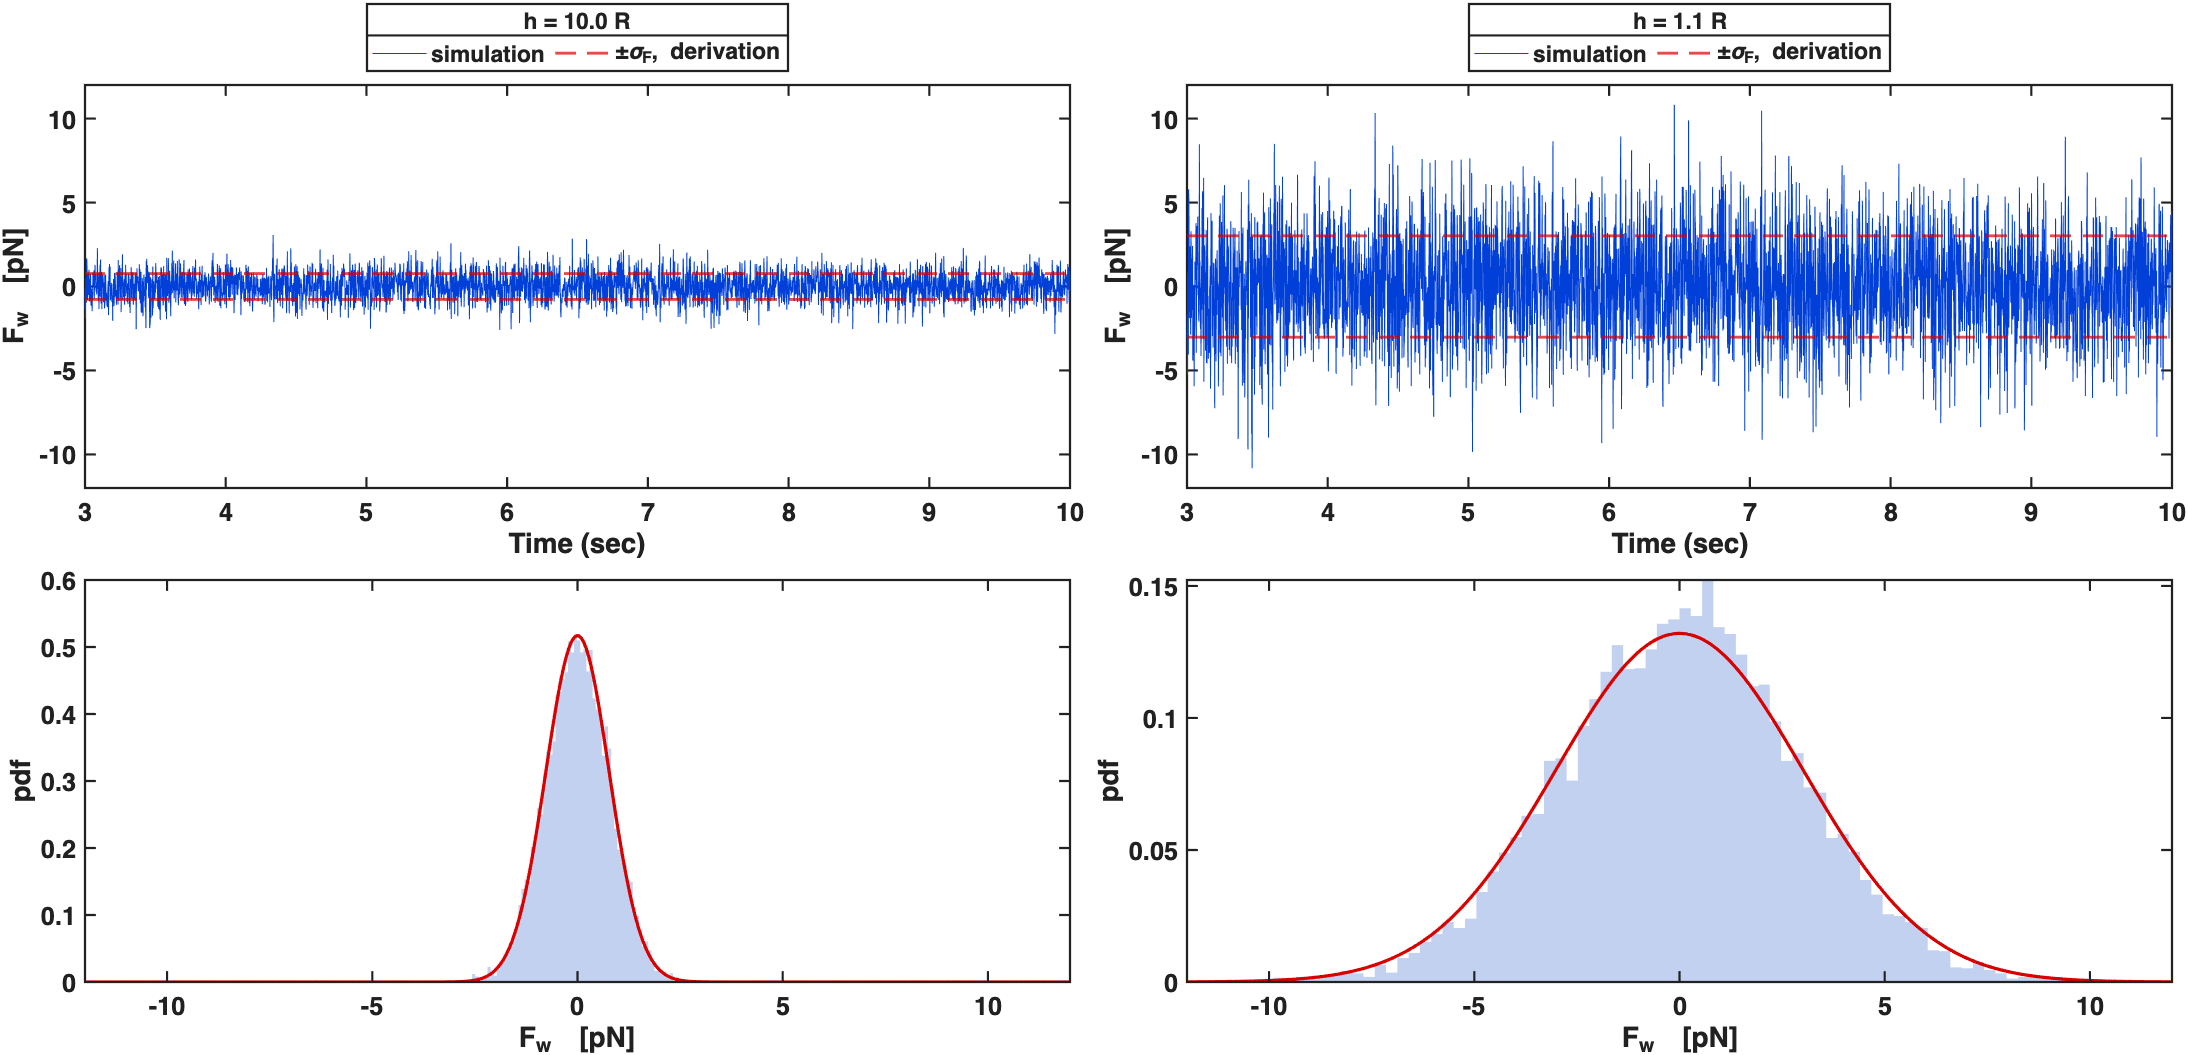
\includegraphics[width=\textwidth]{fig_1104_force_var.png}
\end{center}

\vspace{1.2em}
\begin{center}
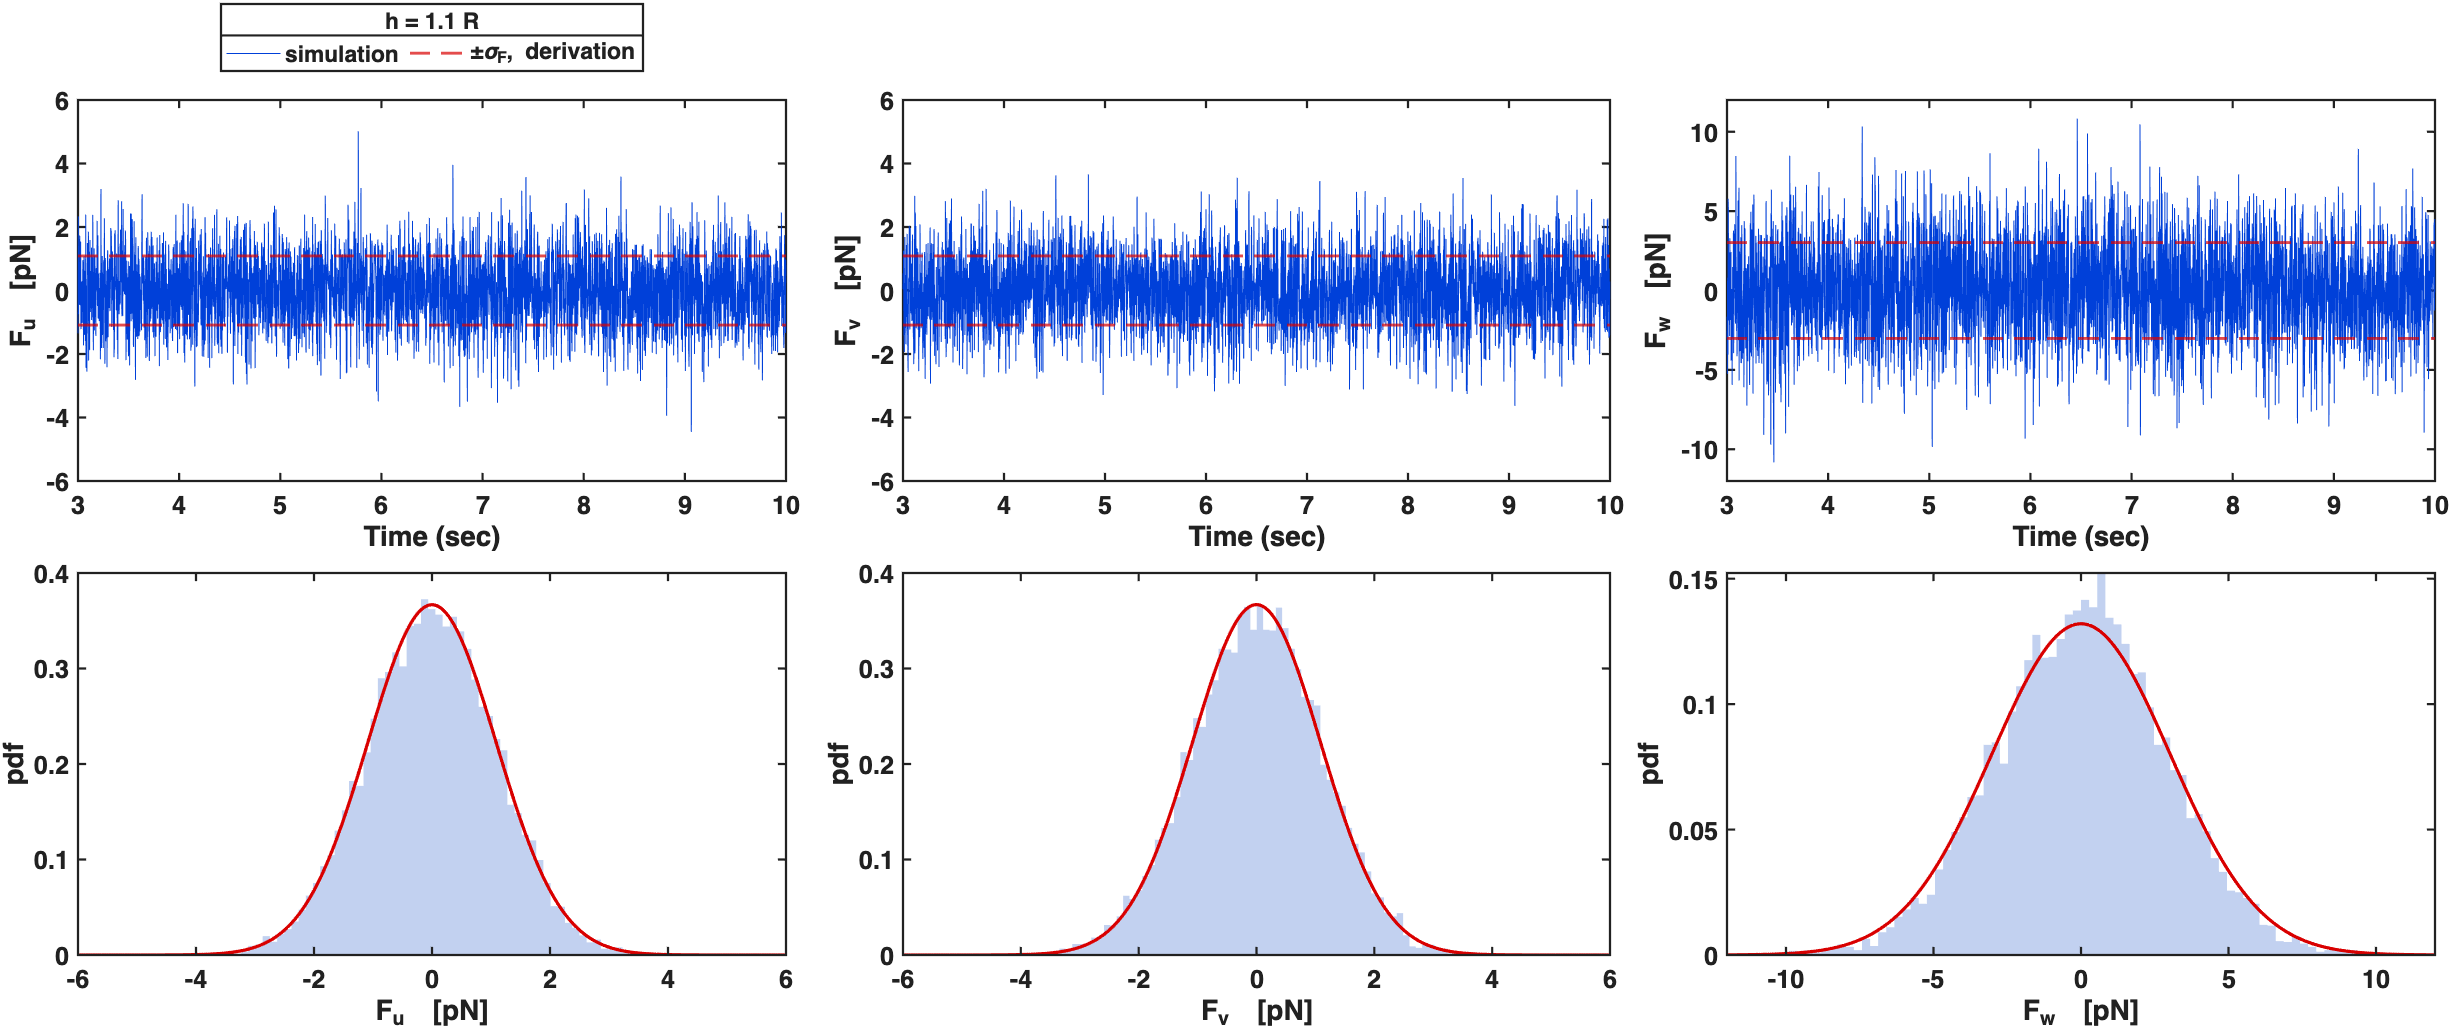
\includegraphics[width=\textwidth]{fig_1104_force_var_uvw.png}
\end{center}

\end{document}
